% Created by tikzDevice version 0.12.3.1 on 2022-08-31 08:56:24
% !TEX encoding = UTF-8 Unicode
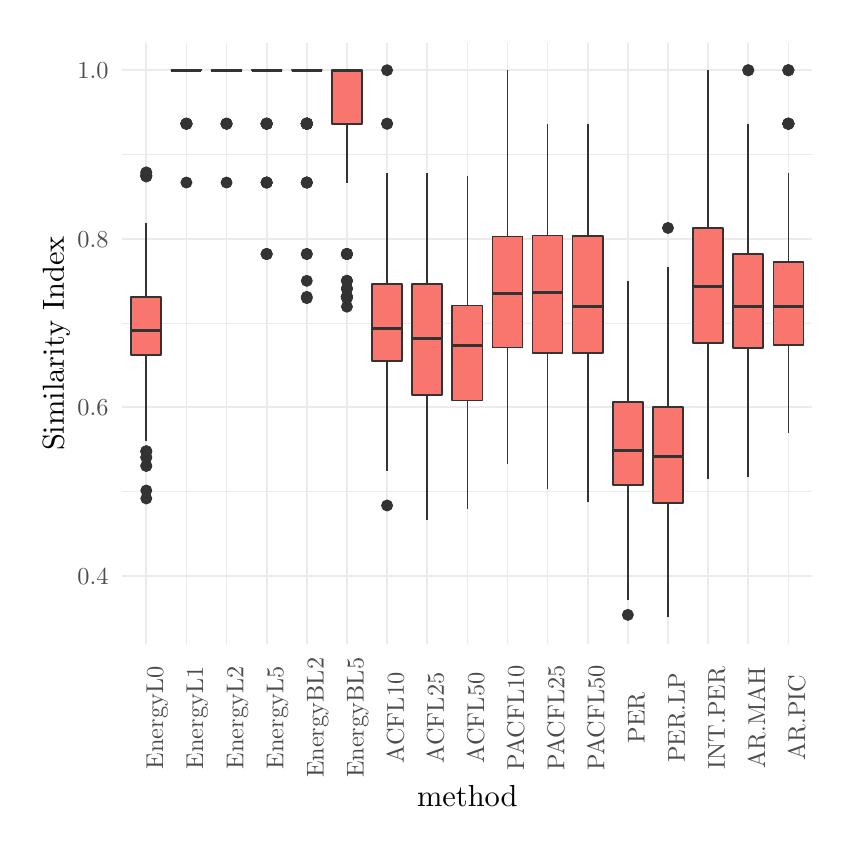
\begin{tikzpicture}[x=1pt,y=1pt]
\definecolor{fillColor}{RGB}{255,255,255}
\path[use as bounding box,fill=fillColor,fill opacity=0.00] (0,0) rectangle (289.08,289.08);
\begin{scope}
\path[clip] ( 34.16, 66.32) rectangle (283.58,283.58);
\definecolor{drawColor}{gray}{0.92}

\path[draw=drawColor,line width= 0.3pt,line join=round] ( 34.16,121.49) --
	(283.58,121.49);

\path[draw=drawColor,line width= 0.3pt,line join=round] ( 34.16,182.38) --
	(283.58,182.38);

\path[draw=drawColor,line width= 0.3pt,line join=round] ( 34.16,243.26) --
	(283.58,243.26);

\path[draw=drawColor,line width= 0.6pt,line join=round] ( 34.16, 91.05) --
	(283.58, 91.05);

\path[draw=drawColor,line width= 0.6pt,line join=round] ( 34.16,151.94) --
	(283.58,151.94);

\path[draw=drawColor,line width= 0.6pt,line join=round] ( 34.16,212.82) --
	(283.58,212.82);

\path[draw=drawColor,line width= 0.6pt,line join=round] ( 34.16,273.70) --
	(283.58,273.70);

\path[draw=drawColor,line width= 0.6pt,line join=round] ( 42.86, 66.32) --
	( 42.86,283.58);

\path[draw=drawColor,line width= 0.6pt,line join=round] ( 57.36, 66.32) --
	( 57.36,283.58);

\path[draw=drawColor,line width= 0.6pt,line join=round] ( 71.86, 66.32) --
	( 71.86,283.58);

\path[draw=drawColor,line width= 0.6pt,line join=round] ( 86.36, 66.32) --
	( 86.36,283.58);

\path[draw=drawColor,line width= 0.6pt,line join=round] (100.86, 66.32) --
	(100.86,283.58);

\path[draw=drawColor,line width= 0.6pt,line join=round] (115.36, 66.32) --
	(115.36,283.58);

\path[draw=drawColor,line width= 0.6pt,line join=round] (129.87, 66.32) --
	(129.87,283.58);

\path[draw=drawColor,line width= 0.6pt,line join=round] (144.37, 66.32) --
	(144.37,283.58);

\path[draw=drawColor,line width= 0.6pt,line join=round] (158.87, 66.32) --
	(158.87,283.58);

\path[draw=drawColor,line width= 0.6pt,line join=round] (173.37, 66.32) --
	(173.37,283.58);

\path[draw=drawColor,line width= 0.6pt,line join=round] (187.87, 66.32) --
	(187.87,283.58);

\path[draw=drawColor,line width= 0.6pt,line join=round] (202.37, 66.32) --
	(202.37,283.58);

\path[draw=drawColor,line width= 0.6pt,line join=round] (216.87, 66.32) --
	(216.87,283.58);

\path[draw=drawColor,line width= 0.6pt,line join=round] (231.37, 66.32) --
	(231.37,283.58);

\path[draw=drawColor,line width= 0.6pt,line join=round] (245.88, 66.32) --
	(245.88,283.58);

\path[draw=drawColor,line width= 0.6pt,line join=round] (260.38, 66.32) --
	(260.38,283.58);

\path[draw=drawColor,line width= 0.6pt,line join=round] (274.88, 66.32) --
	(274.88,283.58);
\definecolor{drawColor}{gray}{0.20}
\definecolor{fillColor}{gray}{0.20}

\path[draw=drawColor,line width= 0.4pt,line join=round,line cap=round,fill=fillColor] ( 42.86,118.96) circle (  1.96);

\path[draw=drawColor,line width= 0.4pt,line join=round,line cap=round,fill=fillColor] ( 42.86,130.74) circle (  1.96);

\path[draw=drawColor,line width= 0.4pt,line join=round,line cap=round,fill=fillColor] ( 42.86,235.65) circle (  1.96);

\path[draw=drawColor,line width= 0.4pt,line join=round,line cap=round,fill=fillColor] ( 42.86,235.35) circle (  1.96);

\path[draw=drawColor,line width= 0.4pt,line join=round,line cap=round,fill=fillColor] ( 42.86,235.65) circle (  1.96);

\path[draw=drawColor,line width= 0.4pt,line join=round,line cap=round,fill=fillColor] ( 42.86,235.65) circle (  1.96);

\path[draw=drawColor,line width= 0.4pt,line join=round,line cap=round,fill=fillColor] ( 42.86,133.82) circle (  1.96);

\path[draw=drawColor,line width= 0.4pt,line join=round,line cap=round,fill=fillColor] ( 42.86,135.99) circle (  1.96);

\path[draw=drawColor,line width= 0.4pt,line join=round,line cap=round,fill=fillColor] ( 42.86,135.99) circle (  1.96);

\path[draw=drawColor,line width= 0.4pt,line join=round,line cap=round,fill=fillColor] ( 42.86,236.74) circle (  1.96);

\path[draw=drawColor,line width= 0.4pt,line join=round,line cap=round,fill=fillColor] ( 42.86,130.74) circle (  1.96);

\path[draw=drawColor,line width= 0.4pt,line join=round,line cap=round,fill=fillColor] ( 42.86,135.99) circle (  1.96);

\path[draw=drawColor,line width= 0.4pt,line join=round,line cap=round,fill=fillColor] ( 42.86,121.83) circle (  1.96);

\path[draw=drawColor,line width= 0.4pt,line join=round,line cap=round,fill=fillColor] ( 42.86,235.35) circle (  1.96);

\path[draw=drawColor,line width= 0.4pt,line join=round,line cap=round,fill=fillColor] ( 42.86,236.74) circle (  1.96);

\path[draw=drawColor,line width= 0.4pt,line join=round,line cap=round,fill=fillColor] ( 42.86,133.82) circle (  1.96);

\path[draw=drawColor,line width= 0.6pt,line join=round] ( 42.86,191.80) -- ( 42.86,218.44);

\path[draw=drawColor,line width= 0.6pt,line join=round] ( 42.86,170.80) -- ( 42.86,139.61);
\definecolor{fillColor}{RGB}{248,118,109}

\path[draw=drawColor,line width= 0.6pt,line join=round,line cap=round,fill=fillColor] ( 37.42,191.80) --
	( 37.42,170.80) --
	( 48.29,170.80) --
	( 48.29,191.80) --
	( 37.42,191.80) --
	cycle;

\path[draw=drawColor,line width= 1.1pt,line join=round] ( 37.42,179.48) -- ( 48.29,179.48);
\definecolor{fillColor}{gray}{0.20}

\path[draw=drawColor,line width= 0.4pt,line join=round,line cap=round,fill=fillColor] ( 57.36,254.38) circle (  1.96);

\path[draw=drawColor,line width= 0.4pt,line join=round,line cap=round,fill=fillColor] ( 57.36,254.38) circle (  1.96);

\path[draw=drawColor,line width= 0.4pt,line join=round,line cap=round,fill=fillColor] ( 57.36,254.38) circle (  1.96);

\path[draw=drawColor,line width= 0.4pt,line join=round,line cap=round,fill=fillColor] ( 57.36,233.11) circle (  1.96);

\path[draw=drawColor,line width= 0.4pt,line join=round,line cap=round,fill=fillColor] ( 57.36,254.38) circle (  1.96);

\path[draw=drawColor,line width= 0.4pt,line join=round,line cap=round,fill=fillColor] ( 57.36,254.38) circle (  1.96);

\path[draw=drawColor,line width= 0.4pt,line join=round,line cap=round,fill=fillColor] ( 57.36,254.38) circle (  1.96);

\path[draw=drawColor,line width= 0.6pt,line join=round] ( 57.36,273.70) -- ( 57.36,273.70);

\path[draw=drawColor,line width= 0.6pt,line join=round] ( 57.36,273.70) -- ( 57.36,273.70);
\definecolor{fillColor}{RGB}{248,118,109}

\path[draw=drawColor,line width= 0.6pt,line join=round,line cap=round,fill=fillColor] ( 51.92,273.70) --
	( 51.92,273.70) --
	( 62.80,273.70) --
	( 62.80,273.70) --
	( 51.92,273.70) --
	cycle;

\path[draw=drawColor,line width= 1.1pt,line join=round] ( 51.92,273.70) -- ( 62.80,273.70);
\definecolor{fillColor}{gray}{0.20}

\path[draw=drawColor,line width= 0.4pt,line join=round,line cap=round,fill=fillColor] ( 71.86,254.38) circle (  1.96);

\path[draw=drawColor,line width= 0.4pt,line join=round,line cap=round,fill=fillColor] ( 71.86,233.11) circle (  1.96);

\path[draw=drawColor,line width= 0.4pt,line join=round,line cap=round,fill=fillColor] ( 71.86,254.38) circle (  1.96);

\path[draw=drawColor,line width= 0.4pt,line join=round,line cap=round,fill=fillColor] ( 71.86,254.38) circle (  1.96);

\path[draw=drawColor,line width= 0.4pt,line join=round,line cap=round,fill=fillColor] ( 71.86,254.38) circle (  1.96);

\path[draw=drawColor,line width= 0.6pt,line join=round] ( 71.86,273.70) -- ( 71.86,273.70);

\path[draw=drawColor,line width= 0.6pt,line join=round] ( 71.86,273.70) -- ( 71.86,273.70);
\definecolor{fillColor}{RGB}{248,118,109}

\path[draw=drawColor,line width= 0.6pt,line join=round,line cap=round,fill=fillColor] ( 66.42,273.70) --
	( 66.42,273.70) --
	( 77.30,273.70) --
	( 77.30,273.70) --
	( 66.42,273.70) --
	cycle;

\path[draw=drawColor,line width= 1.1pt,line join=round] ( 66.42,273.70) -- ( 77.30,273.70);
\definecolor{fillColor}{gray}{0.20}

\path[draw=drawColor,line width= 0.4pt,line join=round,line cap=round,fill=fillColor] ( 86.36,254.38) circle (  1.96);

\path[draw=drawColor,line width= 0.4pt,line join=round,line cap=round,fill=fillColor] ( 86.36,233.11) circle (  1.96);

\path[draw=drawColor,line width= 0.4pt,line join=round,line cap=round,fill=fillColor] ( 86.36,207.29) circle (  1.96);

\path[draw=drawColor,line width= 0.4pt,line join=round,line cap=round,fill=fillColor] ( 86.36,254.38) circle (  1.96);

\path[draw=drawColor,line width= 0.4pt,line join=round,line cap=round,fill=fillColor] ( 86.36,207.29) circle (  1.96);

\path[draw=drawColor,line width= 0.4pt,line join=round,line cap=round,fill=fillColor] ( 86.36,254.38) circle (  1.96);

\path[draw=drawColor,line width= 0.4pt,line join=round,line cap=round,fill=fillColor] ( 86.36,254.38) circle (  1.96);

\path[draw=drawColor,line width= 0.4pt,line join=round,line cap=round,fill=fillColor] ( 86.36,254.38) circle (  1.96);

\path[draw=drawColor,line width= 0.4pt,line join=round,line cap=round,fill=fillColor] ( 86.36,254.38) circle (  1.96);

\path[draw=drawColor,line width= 0.4pt,line join=round,line cap=round,fill=fillColor] ( 86.36,233.11) circle (  1.96);

\path[draw=drawColor,line width= 0.4pt,line join=round,line cap=round,fill=fillColor] ( 86.36,233.11) circle (  1.96);

\path[draw=drawColor,line width= 0.4pt,line join=round,line cap=round,fill=fillColor] ( 86.36,254.38) circle (  1.96);

\path[draw=drawColor,line width= 0.4pt,line join=round,line cap=round,fill=fillColor] ( 86.36,254.38) circle (  1.96);

\path[draw=drawColor,line width= 0.4pt,line join=round,line cap=round,fill=fillColor] ( 86.36,254.38) circle (  1.96);

\path[draw=drawColor,line width= 0.4pt,line join=round,line cap=round,fill=fillColor] ( 86.36,233.11) circle (  1.96);

\path[draw=drawColor,line width= 0.4pt,line join=round,line cap=round,fill=fillColor] ( 86.36,207.29) circle (  1.96);

\path[draw=drawColor,line width= 0.6pt,line join=round] ( 86.36,273.70) -- ( 86.36,273.70);

\path[draw=drawColor,line width= 0.6pt,line join=round] ( 86.36,273.70) -- ( 86.36,273.70);
\definecolor{fillColor}{RGB}{248,118,109}

\path[draw=drawColor,line width= 0.6pt,line join=round,line cap=round,fill=fillColor] ( 80.92,273.70) --
	( 80.92,273.70) --
	( 91.80,273.70) --
	( 91.80,273.70) --
	( 80.92,273.70) --
	cycle;

\path[draw=drawColor,line width= 1.1pt,line join=round] ( 80.92,273.70) -- ( 91.80,273.70);
\definecolor{fillColor}{gray}{0.20}

\path[draw=drawColor,line width= 0.4pt,line join=round,line cap=round,fill=fillColor] (100.86,207.29) circle (  1.96);

\path[draw=drawColor,line width= 0.4pt,line join=round,line cap=round,fill=fillColor] (100.86,254.38) circle (  1.96);

\path[draw=drawColor,line width= 0.4pt,line join=round,line cap=round,fill=fillColor] (100.86,207.29) circle (  1.96);

\path[draw=drawColor,line width= 0.4pt,line join=round,line cap=round,fill=fillColor] (100.86,233.11) circle (  1.96);

\path[draw=drawColor,line width= 0.4pt,line join=round,line cap=round,fill=fillColor] (100.86,254.38) circle (  1.96);

\path[draw=drawColor,line width= 0.4pt,line join=round,line cap=round,fill=fillColor] (100.86,233.11) circle (  1.96);

\path[draw=drawColor,line width= 0.4pt,line join=round,line cap=round,fill=fillColor] (100.86,254.38) circle (  1.96);

\path[draw=drawColor,line width= 0.4pt,line join=round,line cap=round,fill=fillColor] (100.86,197.60) circle (  1.96);

\path[draw=drawColor,line width= 0.4pt,line join=round,line cap=round,fill=fillColor] (100.86,254.38) circle (  1.96);

\path[draw=drawColor,line width= 0.4pt,line join=round,line cap=round,fill=fillColor] (100.86,191.34) circle (  1.96);

\path[draw=drawColor,line width= 0.4pt,line join=round,line cap=round,fill=fillColor] (100.86,254.38) circle (  1.96);

\path[draw=drawColor,line width= 0.4pt,line join=round,line cap=round,fill=fillColor] (100.86,254.38) circle (  1.96);

\path[draw=drawColor,line width= 0.4pt,line join=round,line cap=round,fill=fillColor] (100.86,254.38) circle (  1.96);

\path[draw=drawColor,line width= 0.4pt,line join=round,line cap=round,fill=fillColor] (100.86,254.38) circle (  1.96);

\path[draw=drawColor,line width= 0.4pt,line join=round,line cap=round,fill=fillColor] (100.86,233.11) circle (  1.96);

\path[draw=drawColor,line width= 0.4pt,line join=round,line cap=round,fill=fillColor] (100.86,191.80) circle (  1.96);

\path[draw=drawColor,line width= 0.4pt,line join=round,line cap=round,fill=fillColor] (100.86,254.38) circle (  1.96);

\path[draw=drawColor,line width= 0.4pt,line join=round,line cap=round,fill=fillColor] (100.86,254.38) circle (  1.96);

\path[draw=drawColor,line width= 0.4pt,line join=round,line cap=round,fill=fillColor] (100.86,254.38) circle (  1.96);

\path[draw=drawColor,line width= 0.4pt,line join=round,line cap=round,fill=fillColor] (100.86,254.38) circle (  1.96);

\path[draw=drawColor,line width= 0.4pt,line join=round,line cap=round,fill=fillColor] (100.86,254.38) circle (  1.96);

\path[draw=drawColor,line width= 0.4pt,line join=round,line cap=round,fill=fillColor] (100.86,254.38) circle (  1.96);

\path[draw=drawColor,line width= 0.4pt,line join=round,line cap=round,fill=fillColor] (100.86,254.38) circle (  1.96);

\path[draw=drawColor,line width= 0.4pt,line join=round,line cap=round,fill=fillColor] (100.86,254.38) circle (  1.96);

\path[draw=drawColor,line width= 0.4pt,line join=round,line cap=round,fill=fillColor] (100.86,233.11) circle (  1.96);

\path[draw=drawColor,line width= 0.4pt,line join=round,line cap=round,fill=fillColor] (100.86,254.38) circle (  1.96);

\path[draw=drawColor,line width= 0.4pt,line join=round,line cap=round,fill=fillColor] (100.86,254.38) circle (  1.96);

\path[draw=drawColor,line width= 0.4pt,line join=round,line cap=round,fill=fillColor] (100.86,254.38) circle (  1.96);

\path[draw=drawColor,line width= 0.4pt,line join=round,line cap=round,fill=fillColor] (100.86,254.38) circle (  1.96);

\path[draw=drawColor,line width= 0.6pt,line join=round] (100.86,273.70) -- (100.86,273.70);

\path[draw=drawColor,line width= 0.6pt,line join=round] (100.86,273.70) -- (100.86,273.70);
\definecolor{fillColor}{RGB}{248,118,109}

\path[draw=drawColor,line width= 0.6pt,line join=round,line cap=round,fill=fillColor] ( 95.42,273.70) --
	( 95.42,273.70) --
	(106.30,273.70) --
	(106.30,273.70) --
	( 95.42,273.70) --
	cycle;

\path[draw=drawColor,line width= 1.1pt,line join=round] ( 95.42,273.70) -- (106.30,273.70);
\definecolor{fillColor}{gray}{0.20}

\path[draw=drawColor,line width= 0.4pt,line join=round,line cap=round,fill=fillColor] (115.36,207.29) circle (  1.96);

\path[draw=drawColor,line width= 0.4pt,line join=round,line cap=round,fill=fillColor] (115.36,207.29) circle (  1.96);

\path[draw=drawColor,line width= 0.4pt,line join=round,line cap=round,fill=fillColor] (115.36,191.80) circle (  1.96);

\path[draw=drawColor,line width= 0.4pt,line join=round,line cap=round,fill=fillColor] (115.36,197.60) circle (  1.96);

\path[draw=drawColor,line width= 0.4pt,line join=round,line cap=round,fill=fillColor] (115.36,191.80) circle (  1.96);

\path[draw=drawColor,line width= 0.4pt,line join=round,line cap=round,fill=fillColor] (115.36,194.58) circle (  1.96);

\path[draw=drawColor,line width= 0.4pt,line join=round,line cap=round,fill=fillColor] (115.36,207.29) circle (  1.96);

\path[draw=drawColor,line width= 0.4pt,line join=round,line cap=round,fill=fillColor] (115.36,188.26) circle (  1.96);

\path[draw=drawColor,line width= 0.4pt,line join=round,line cap=round,fill=fillColor] (115.36,194.96) circle (  1.96);

\path[draw=drawColor,line width= 0.4pt,line join=round,line cap=round,fill=fillColor] (115.36,191.80) circle (  1.96);

\path[draw=drawColor,line width= 0.4pt,line join=round,line cap=round,fill=fillColor] (115.36,191.80) circle (  1.96);

\path[draw=drawColor,line width= 0.4pt,line join=round,line cap=round,fill=fillColor] (115.36,207.29) circle (  1.96);

\path[draw=drawColor,line width= 0.4pt,line join=round,line cap=round,fill=fillColor] (115.36,207.29) circle (  1.96);

\path[draw=drawColor,line width= 0.4pt,line join=round,line cap=round,fill=fillColor] (115.36,191.80) circle (  1.96);

\path[draw=drawColor,line width= 0.4pt,line join=round,line cap=round,fill=fillColor] (115.36,197.60) circle (  1.96);

\path[draw=drawColor,line width= 0.4pt,line join=round,line cap=round,fill=fillColor] (115.36,197.60) circle (  1.96);

\path[draw=drawColor,line width= 0.4pt,line join=round,line cap=round,fill=fillColor] (115.36,191.34) circle (  1.96);

\path[draw=drawColor,line width= 0.4pt,line join=round,line cap=round,fill=fillColor] (115.36,207.29) circle (  1.96);

\path[draw=drawColor,line width= 0.4pt,line join=round,line cap=round,fill=fillColor] (115.36,191.80) circle (  1.96);

\path[draw=drawColor,line width= 0.4pt,line join=round,line cap=round,fill=fillColor] (115.36,191.80) circle (  1.96);

\path[draw=drawColor,line width= 0.4pt,line join=round,line cap=round,fill=fillColor] (115.36,191.80) circle (  1.96);

\path[draw=drawColor,line width= 0.4pt,line join=round,line cap=round,fill=fillColor] (115.36,191.80) circle (  1.96);

\path[draw=drawColor,line width= 0.4pt,line join=round,line cap=round,fill=fillColor] (115.36,191.80) circle (  1.96);

\path[draw=drawColor,line width= 0.6pt,line join=round] (115.36,273.70) -- (115.36,273.70);

\path[draw=drawColor,line width= 0.6pt,line join=round] (115.36,254.38) -- (115.36,233.11);
\definecolor{fillColor}{RGB}{248,118,109}

\path[draw=drawColor,line width= 0.6pt,line join=round,line cap=round,fill=fillColor] (109.93,273.70) --
	(109.93,254.38) --
	(120.80,254.38) --
	(120.80,273.70) --
	(109.93,273.70) --
	cycle;

\path[draw=drawColor,line width= 1.1pt,line join=round] (109.93,273.70) -- (120.80,273.70);
\definecolor{fillColor}{gray}{0.20}

\path[draw=drawColor,line width= 0.4pt,line join=round,line cap=round,fill=fillColor] (129.87,254.38) circle (  1.96);

\path[draw=drawColor,line width= 0.4pt,line join=round,line cap=round,fill=fillColor] (129.87,254.38) circle (  1.96);

\path[draw=drawColor,line width= 0.4pt,line join=round,line cap=round,fill=fillColor] (129.87,273.70) circle (  1.96);

\path[draw=drawColor,line width= 0.4pt,line join=round,line cap=round,fill=fillColor] (129.87,116.42) circle (  1.96);

\path[draw=drawColor,line width= 0.6pt,line join=round] (129.87,196.39) -- (129.87,236.74);

\path[draw=drawColor,line width= 0.6pt,line join=round] (129.87,168.64) -- (129.87,129.01);
\definecolor{fillColor}{RGB}{248,118,109}

\path[draw=drawColor,line width= 0.6pt,line join=round,line cap=round,fill=fillColor] (124.43,196.39) --
	(124.43,168.64) --
	(135.30,168.64) --
	(135.30,196.39) --
	(124.43,196.39) --
	cycle;

\path[draw=drawColor,line width= 1.1pt,line join=round] (124.43,180.32) -- (135.30,180.32);

\path[draw=drawColor,line width= 0.6pt,line join=round] (144.37,196.39) -- (144.37,236.74);

\path[draw=drawColor,line width= 0.6pt,line join=round] (144.37,156.28) -- (144.37,111.35);

\path[draw=drawColor,line width= 0.6pt,line join=round,line cap=round,fill=fillColor] (138.93,196.39) --
	(138.93,156.28) --
	(149.80,156.28) --
	(149.80,196.39) --
	(138.93,196.39) --
	cycle;

\path[draw=drawColor,line width= 1.1pt,line join=round] (138.93,176.64) -- (149.80,176.64);

\path[draw=drawColor,line width= 0.6pt,line join=round] (158.87,188.72) -- (158.87,235.35);

\path[draw=drawColor,line width= 0.6pt,line join=round] (158.87,154.31) -- (158.87,115.15);

\path[draw=drawColor,line width= 0.6pt,line join=round,line cap=round,fill=fillColor] (153.43,188.72) --
	(153.43,154.31) --
	(164.31,154.31) --
	(164.31,188.72) --
	(153.43,188.72) --
	cycle;

\path[draw=drawColor,line width= 1.1pt,line join=round] (153.43,174.07) -- (164.31,174.07);

\path[draw=drawColor,line width= 0.6pt,line join=round] (173.37,213.65) -- (173.37,273.70);

\path[draw=drawColor,line width= 0.6pt,line join=round] (173.37,173.47) -- (173.37,131.54);

\path[draw=drawColor,line width= 0.6pt,line join=round,line cap=round,fill=fillColor] (167.93,213.65) --
	(167.93,173.47) --
	(178.81,173.47) --
	(178.81,213.65) --
	(167.93,213.65) --
	cycle;

\path[draw=drawColor,line width= 1.1pt,line join=round] (167.93,192.89) -- (178.81,192.89);

\path[draw=drawColor,line width= 0.6pt,line join=round] (187.87,213.97) -- (187.87,254.38);

\path[draw=drawColor,line width= 0.6pt,line join=round] (187.87,171.51) -- (187.87,122.34);

\path[draw=drawColor,line width= 0.6pt,line join=round,line cap=round,fill=fillColor] (182.43,213.97) --
	(182.43,171.51) --
	(193.31,171.51) --
	(193.31,213.97) --
	(182.43,213.97) --
	cycle;

\path[draw=drawColor,line width= 1.1pt,line join=round] (182.43,193.25) -- (193.31,193.25);

\path[draw=drawColor,line width= 0.6pt,line join=round] (202.37,213.79) -- (202.37,254.38);

\path[draw=drawColor,line width= 0.6pt,line join=round] (202.37,171.51) -- (202.37,117.70);

\path[draw=drawColor,line width= 0.6pt,line join=round,line cap=round,fill=fillColor] (196.93,213.79) --
	(196.93,171.51) --
	(207.81,171.51) --
	(207.81,213.79) --
	(196.93,213.79) --
	cycle;

\path[draw=drawColor,line width= 1.1pt,line join=round] (196.93,188.49) -- (207.81,188.49);
\definecolor{fillColor}{gray}{0.20}

\path[draw=drawColor,line width= 0.4pt,line join=round,line cap=round,fill=fillColor] (216.87, 76.89) circle (  1.96);

\path[draw=drawColor,line width= 0.6pt,line join=round] (216.87,153.84) -- (216.87,197.68);

\path[draw=drawColor,line width= 0.6pt,line join=round] (216.87,123.84) -- (216.87, 82.35);
\definecolor{fillColor}{RGB}{248,118,109}

\path[draw=drawColor,line width= 0.6pt,line join=round,line cap=round,fill=fillColor] (211.44,153.84) --
	(211.44,123.84) --
	(222.31,123.84) --
	(222.31,153.84) --
	(211.44,153.84) --
	cycle;

\path[draw=drawColor,line width= 1.1pt,line join=round] (211.44,136.35) -- (222.31,136.35);
\definecolor{fillColor}{gray}{0.20}

\path[draw=drawColor,line width= 0.4pt,line join=round,line cap=round,fill=fillColor] (231.37,216.71) circle (  1.96);

\path[draw=drawColor,line width= 0.6pt,line join=round] (231.37,152.05) -- (231.37,202.49);

\path[draw=drawColor,line width= 0.6pt,line join=round] (231.37,117.34) -- (231.37, 76.19);
\definecolor{fillColor}{RGB}{248,118,109}

\path[draw=drawColor,line width= 0.6pt,line join=round,line cap=round,fill=fillColor] (225.94,152.05) --
	(225.94,117.34) --
	(236.81,117.34) --
	(236.81,152.05) --
	(225.94,152.05) --
	cycle;

\path[draw=drawColor,line width= 1.1pt,line join=round] (225.94,134.18) -- (236.81,134.18);

\path[draw=drawColor,line width= 0.6pt,line join=round] (245.88,216.71) -- (245.88,273.70);

\path[draw=drawColor,line width= 0.6pt,line join=round] (245.88,175.13) -- (245.88,126.11);

\path[draw=drawColor,line width= 0.6pt,line join=round,line cap=round,fill=fillColor] (240.44,216.71) --
	(240.44,175.13) --
	(251.31,175.13) --
	(251.31,216.71) --
	(240.44,216.71) --
	cycle;

\path[draw=drawColor,line width= 1.1pt,line join=round] (240.44,195.49) -- (251.31,195.49);
\definecolor{fillColor}{gray}{0.20}

\path[draw=drawColor,line width= 0.4pt,line join=round,line cap=round,fill=fillColor] (260.38,273.70) circle (  1.96);

\path[draw=drawColor,line width= 0.4pt,line join=round,line cap=round,fill=fillColor] (260.38,273.70) circle (  1.96);

\path[draw=drawColor,line width= 0.6pt,line join=round] (260.38,207.29) -- (260.38,254.38);

\path[draw=drawColor,line width= 0.6pt,line join=round] (260.38,173.35) -- (260.38,126.57);
\definecolor{fillColor}{RGB}{248,118,109}

\path[draw=drawColor,line width= 0.6pt,line join=round,line cap=round,fill=fillColor] (254.94,207.29) --
	(254.94,173.35) --
	(265.82,173.35) --
	(265.82,207.29) --
	(254.94,207.29) --
	cycle;

\path[draw=drawColor,line width= 1.1pt,line join=round] (254.94,188.26) -- (265.82,188.26);
\definecolor{fillColor}{gray}{0.20}

\path[draw=drawColor,line width= 0.4pt,line join=round,line cap=round,fill=fillColor] (274.88,254.38) circle (  1.96);

\path[draw=drawColor,line width= 0.4pt,line join=round,line cap=round,fill=fillColor] (274.88,273.70) circle (  1.96);

\path[draw=drawColor,line width= 0.4pt,line join=round,line cap=round,fill=fillColor] (274.88,254.38) circle (  1.96);

\path[draw=drawColor,line width= 0.4pt,line join=round,line cap=round,fill=fillColor] (274.88,254.38) circle (  1.96);

\path[draw=drawColor,line width= 0.4pt,line join=round,line cap=round,fill=fillColor] (274.88,254.38) circle (  1.96);

\path[draw=drawColor,line width= 0.4pt,line join=round,line cap=round,fill=fillColor] (274.88,273.70) circle (  1.96);

\path[draw=drawColor,line width= 0.4pt,line join=round,line cap=round,fill=fillColor] (274.88,254.38) circle (  1.96);

\path[draw=drawColor,line width= 0.4pt,line join=round,line cap=round,fill=fillColor] (274.88,254.38) circle (  1.96);

\path[draw=drawColor,line width= 0.4pt,line join=round,line cap=round,fill=fillColor] (274.88,254.38) circle (  1.96);

\path[draw=drawColor,line width= 0.4pt,line join=round,line cap=round,fill=fillColor] (274.88,254.38) circle (  1.96);

\path[draw=drawColor,line width= 0.4pt,line join=round,line cap=round,fill=fillColor] (274.88,273.70) circle (  1.96);

\path[draw=drawColor,line width= 0.6pt,line join=round] (274.88,204.36) -- (274.88,236.74);

\path[draw=drawColor,line width= 0.6pt,line join=round] (274.88,174.37) -- (274.88,142.63);
\definecolor{fillColor}{RGB}{248,118,109}

\path[draw=drawColor,line width= 0.6pt,line join=round,line cap=round,fill=fillColor] (269.44,204.36) --
	(269.44,174.37) --
	(280.32,174.37) --
	(280.32,204.36) --
	(269.44,204.36) --
	cycle;

\path[draw=drawColor,line width= 1.1pt,line join=round] (269.44,188.26) -- (280.32,188.26);
\end{scope}
\begin{scope}
\path[clip] (  0.00,  0.00) rectangle (289.08,289.08);
\definecolor{drawColor}{gray}{0.30}

\node[text=drawColor,anchor=base east,inner sep=0pt, outer sep=0pt, scale=  0.88] at ( 29.21, 88.02) {0.4};

\node[text=drawColor,anchor=base east,inner sep=0pt, outer sep=0pt, scale=  0.88] at ( 29.21,148.91) {0.6};

\node[text=drawColor,anchor=base east,inner sep=0pt, outer sep=0pt, scale=  0.88] at ( 29.21,209.79) {0.8};

\node[text=drawColor,anchor=base east,inner sep=0pt, outer sep=0pt, scale=  0.88] at ( 29.21,270.67) {1.0};
\end{scope}
\begin{scope}
\path[clip] (  0.00,  0.00) rectangle (289.08,289.08);
\definecolor{drawColor}{gray}{0.30}

\node[text=drawColor,rotate= 90.00,anchor=base,inner sep=0pt, outer sep=0pt, scale=  0.88] at ( 48.92, 39.67) {EnergyL0};

\node[text=drawColor,rotate= 90.00,anchor=base,inner sep=0pt, outer sep=0pt, scale=  0.88] at ( 63.42, 39.67) {EnergyL1};

\node[text=drawColor,rotate= 90.00,anchor=base,inner sep=0pt, outer sep=0pt, scale=  0.88] at ( 77.92, 39.67) {EnergyL2};

\node[text=drawColor,rotate= 90.00,anchor=base,inner sep=0pt, outer sep=0pt, scale=  0.88] at ( 92.42, 39.67) {EnergyL5};

\node[text=drawColor,rotate= 90.00,anchor=base,inner sep=0pt, outer sep=0pt, scale=  0.88] at (106.92, 39.67) {EnergyBL2};

\node[text=drawColor,rotate= 90.00,anchor=base,inner sep=0pt, outer sep=0pt, scale=  0.88] at (121.42, 39.67) {EnergyBL5};

\node[text=drawColor,rotate= 90.00,anchor=base,inner sep=0pt, outer sep=0pt, scale=  0.88] at (135.93, 39.67) {ACFL10};

\node[text=drawColor,rotate= 90.00,anchor=base,inner sep=0pt, outer sep=0pt, scale=  0.88] at (150.43, 39.67) {ACFL25};

\node[text=drawColor,rotate= 90.00,anchor=base,inner sep=0pt, outer sep=0pt, scale=  0.88] at (164.93, 39.67) {ACFL50};

\node[text=drawColor,rotate= 90.00,anchor=base,inner sep=0pt, outer sep=0pt, scale=  0.88] at (179.43, 39.67) {PACFL10};

\node[text=drawColor,rotate= 90.00,anchor=base,inner sep=0pt, outer sep=0pt, scale=  0.88] at (193.93, 39.67) {PACFL25};

\node[text=drawColor,rotate= 90.00,anchor=base,inner sep=0pt, outer sep=0pt, scale=  0.88] at (208.43, 39.67) {PACFL50};

\node[text=drawColor,rotate= 90.00,anchor=base,inner sep=0pt, outer sep=0pt, scale=  0.88] at (222.93, 39.67) {PER};

\node[text=drawColor,rotate= 90.00,anchor=base,inner sep=0pt, outer sep=0pt, scale=  0.88] at (237.44, 39.67) {PER.LP};

\node[text=drawColor,rotate= 90.00,anchor=base,inner sep=0pt, outer sep=0pt, scale=  0.88] at (251.94, 39.67) {INT.PER};

\node[text=drawColor,rotate= 90.00,anchor=base,inner sep=0pt, outer sep=0pt, scale=  0.88] at (266.44, 39.67) {AR.MAH};

\node[text=drawColor,rotate= 90.00,anchor=base,inner sep=0pt, outer sep=0pt, scale=  0.88] at (280.94, 39.67) {AR.PIC};
\end{scope}
\begin{scope}
\path[clip] (  0.00,  0.00) rectangle (289.08,289.08);
\definecolor{drawColor}{RGB}{0,0,0}

\node[text=drawColor,anchor=base,inner sep=0pt, outer sep=0pt, scale=  1.10] at (158.87,  7.64) {method};
\end{scope}
\begin{scope}
\path[clip] (  0.00,  0.00) rectangle (289.08,289.08);
\definecolor{drawColor}{RGB}{0,0,0}

\node[text=drawColor,rotate= 90.00,anchor=base,inner sep=0pt, outer sep=0pt, scale=  1.10] at ( 13.08,174.95) {Similarity Index};
\end{scope}
\end{tikzpicture}
